\documentclass[xcolor=dvipsnames]{beamer}
\usepackage[utf8]{inputenc}
\usepackage[IL2]{fontenc}
\usepackage[czech]{babel}
\usepackage{float}
\usepackage{listings}
\usepackage{amssymb}
\usepackage{amsmath}
\usepackage{mathtools}
\usepackage{url}
\usepackage{graphicx}
\usepackage{subfigure}
%\useoutertheme[subsection=false]{smoothbars}
\usetheme{Madrid}
\usecolortheme[named=OliveGreen]{structure}
%\usecolortheme[named=OliveGreen]{structure} 
%\usetheme[height=7mm]{Rochester} 
%\setbeamertemplate{items}[ball] 
%\setbeamertemplate{blocks}[rounded][shadow=true] 
%\useoutertheme{umbcfootline}
\title{Teorie portfolia}
\author{Marek Bryša, Jan Kovář}
\institute
{
Masarykova Univerzita\\
Přírodovědecká fakulta
}
\date{\today}

\begin{document}
  \frame{\titlepage}
  \section{Teoretická část}
  \documentclass[12pt,a4paper]{article}
\usepackage[utf8]{inputenc}
\usepackage{czech}
\usepackage{amsmath,amssymb,amscd}
\usepackage{graphicx}
\usepackage[top=2cm, bottom=2cm, left=2cm, right=2cm]{geometry}
\usepackage{paralist}
\usepackage{url}

\begin{document}
\thispagestyle{empty}
\vfill
\begin{center}
{\Large \bf Masarykova univerzita\\[1ex]}
{\large Přírodovědecká fakulta}
\end{center}
\vfill
\begin{center}

\includegraphics[scale=0.7]{prf_logo.pdf}
\end{center}
\begin{center}
\vfill

Marek Bryša, Jan Kovář\\[3em]
{\LARGE \bf Kolektivní investování}\\[1em]
SEMINĂ
  \section{Praktická část}
  \begin{frame}{Využitý software}
  \begin{itemize}
    \item
      Skript v Pythonu a NumPy, je rozšířenou a opravenou verzí originálu Travise Vaughta\cite{tvaught}
    \item
      Založen na MPT, historické metodě a metrikách z CAPM, výpočet probíhá numericky iterativně podle práce Williama Sharpa\cite{sharpe}
    \item
      Zdrojem dat je Yahoo! Fiance\cite{yahoo}
    \item
      Výhradně akcie z S\&P500 v období 1.1.2010 až 1.11.2011
    \item
      Tolerance k risku=0.05, bezrizikové aktivum ma nulový výnos, není povolen obchod na krátko
  \end{itemize}
\end{frame}

\begin{frame}{Portfolio výrobců hardware}
      \begin{tabular}{|l|l|r|r|}
        \hline
        Symbol&Název&Volatilita&Roční výnos\\\hline\hline
        A&Agilent Technologies &0.402&16.43\%\\\hline
        AAPL&Apple Inc. &0.266&37.57\%\\\hline
        AMD&Advanced Micro Devices &0.497&-16.46\%\\\hline
        DELL&Dell Inc. &0.345&9.585\%\\\hline
        HPQ&Hewlett-Packard &0.334&-31.4\%\\\hline
        IBM&International Bus. Machines &0.198&20.96\%\\\hline
        INTC&Intel Corp. &0.254&14.2\%\\\hline
        NVDA&Nvidia Corporation &0.512&-0.09651\%\\\hline
        TXN&Texas Instruments &0.267&13.72\%\\\hline
      \end{tabular}
\end{frame}

\begin{frame}{Portfolio výrobců hardware}
        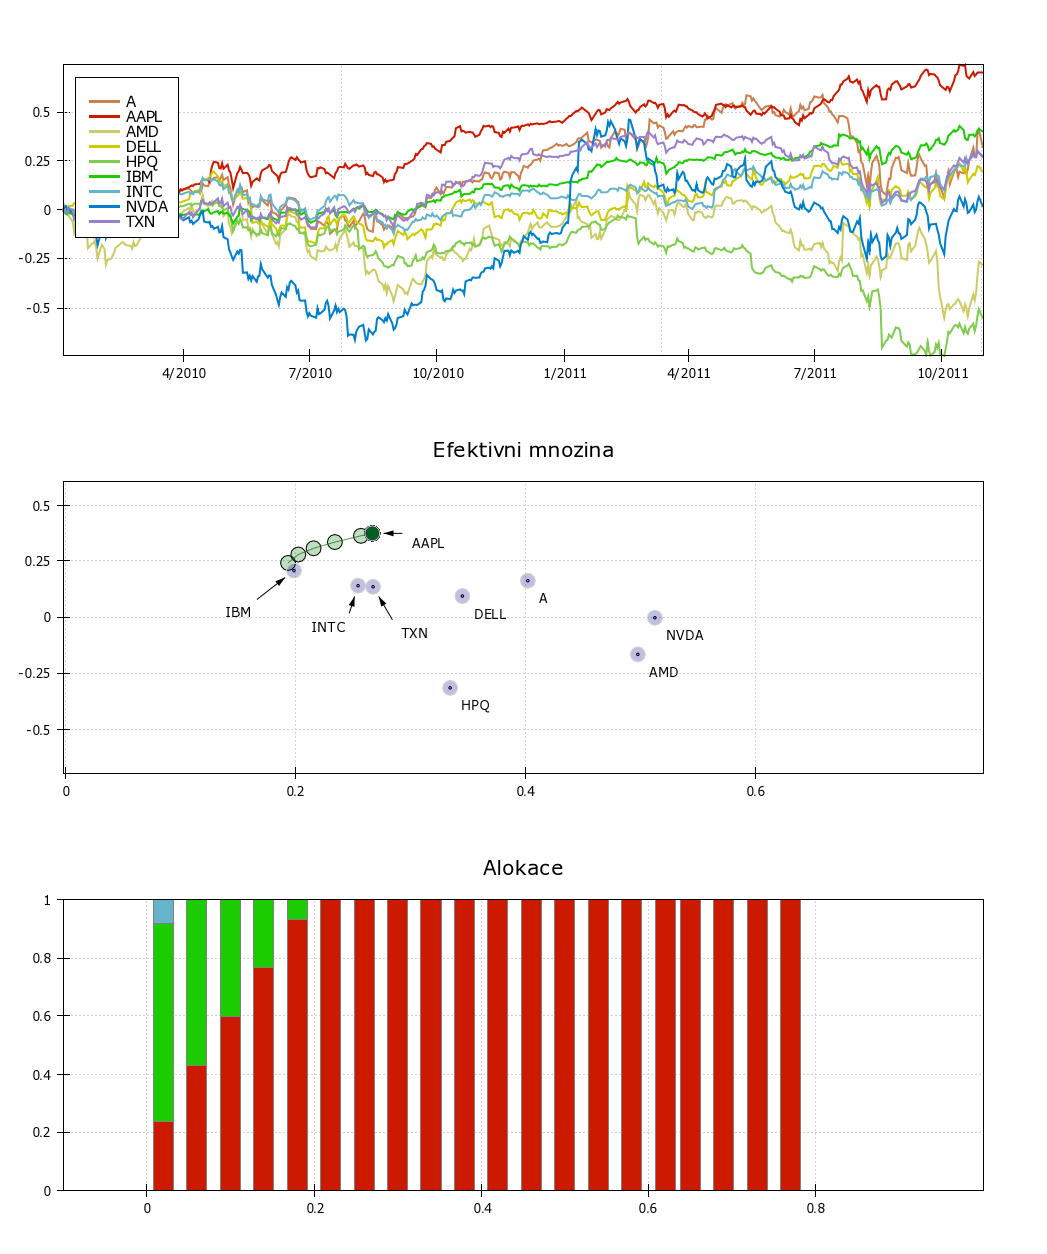
\includegraphics[height=0.9\textheight]{hw1.png}
\end{frame}

\begin{frame}{Portfolio výrobců hardware}
      \begin{tabular}{|l|l|r|}
        \hline
        Symbol&Název&Alokace\\\hline\hline
        AAPL&Apple Inc. &0.346\\\hline
        IBM&International Bus. Machines &0.648\\\hline
        INTC&Intel Corp. &0.0069\\\hline
      \end{tabular}
      
      Výnos 24.37\%\\
      Volatilita 0.193
\end{frame}

\begin{frame}{Portfolio výrobců software}
      \begin{tabular}{|l|l|r|r|}
        \hline
        Symbol&Název&Volatilita&Roční výnos\\\hline\hline
        ADBE&Adobe Systems &0.356&-7.255\%\\\hline
        ADSK&Autodesk Inc. &0.397&23.36\%\\\hline
        AKAM&Akamai Technologies Inc &0.478&12.77\%\\\hline
        EBAY&eBay Inc. &0.35&20.87\%\\\hline
        ERTS&Electronic Arts &0.362&19.38\%\\\hline
        GOOG&Google Inc. &0.291&0.1524\%\\\hline
        MSFT&Microsoft Corp. &0.226&-4.513\%\\\hline
        ORCL&Oracle Corp. &0.287&19.16\%\\\hline
        SYMC&Symantec Corp. &0.306&-0.5626\%\\\hline
        YHOO&Yahoo Inc. &0.351&0.2939\%\\\hline
      \end{tabular}
\end{frame}

\begin{frame}{Portfolio výrobců software}
        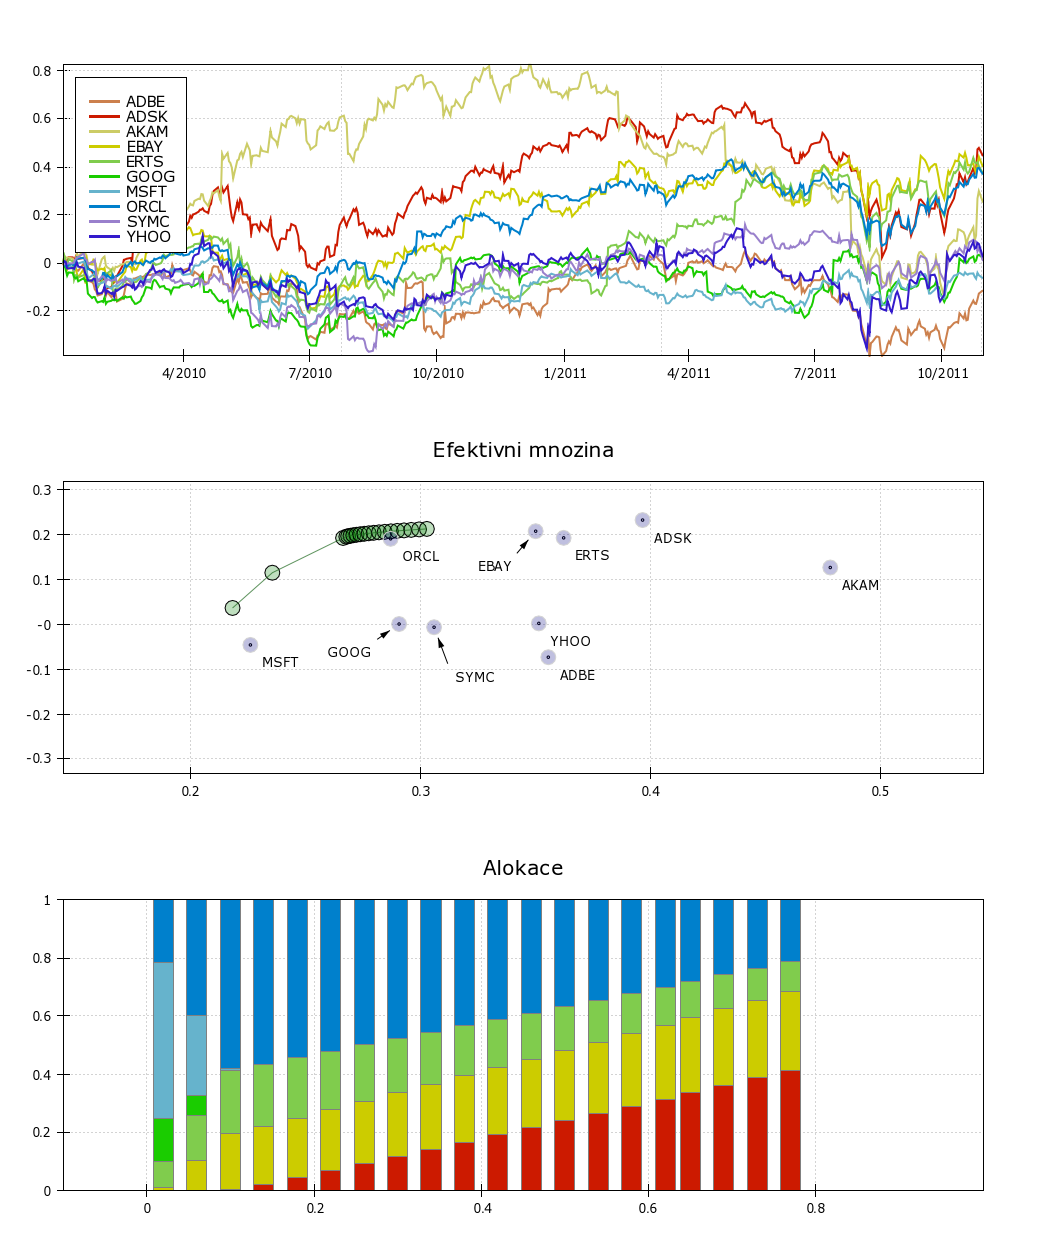
\includegraphics[height=0.9\textheight]{sw1.png}
\end{frame}

\begin{frame}{Portfolio výrobců software}
      \begin{tabular}{|l|l|r|}
        \hline
        Symbol&Název&Alokace\\\hline\hline
        EBAY&eBay Inc. &0.0129\\\hline
        ERTS&Electronic Arts &0.0888\\\hline
        GOOG&Google Inc. &0.149\\\hline
        MSFT&Microsoft Corp. &0.534\\\hline
        ORCL&Oracle Corp. &0.216\\\hline
      \end{tabular}
      
      Výnos 3.736\%\\
      Volatilita 0.218
\end{frame}

\begin{frame}{Portfolio výrobců farmaceutik}
      \begin{tabular}{|l|l|r|r|}
        \hline
        Symbol&Název&Volatilita&Roční výnos\\\hline\hline
        ABT&Abbott Labs &0.16&3.525\%\\\hline
        BAX&Baxter International Inc. &0.244&1.14\%\\\hline
        JNJ&Johnson \& Johnson &0.15&3.236\%\\\hline
        MRK&Merck \& Co. &0.213&1.664\%\\\hline
        PFE&Pfizer Inc. &0.226&6.494\%\\\hline
      \end{tabular}
\end{frame}

\begin{frame}{Portfolio výrobců farmaceutik}
        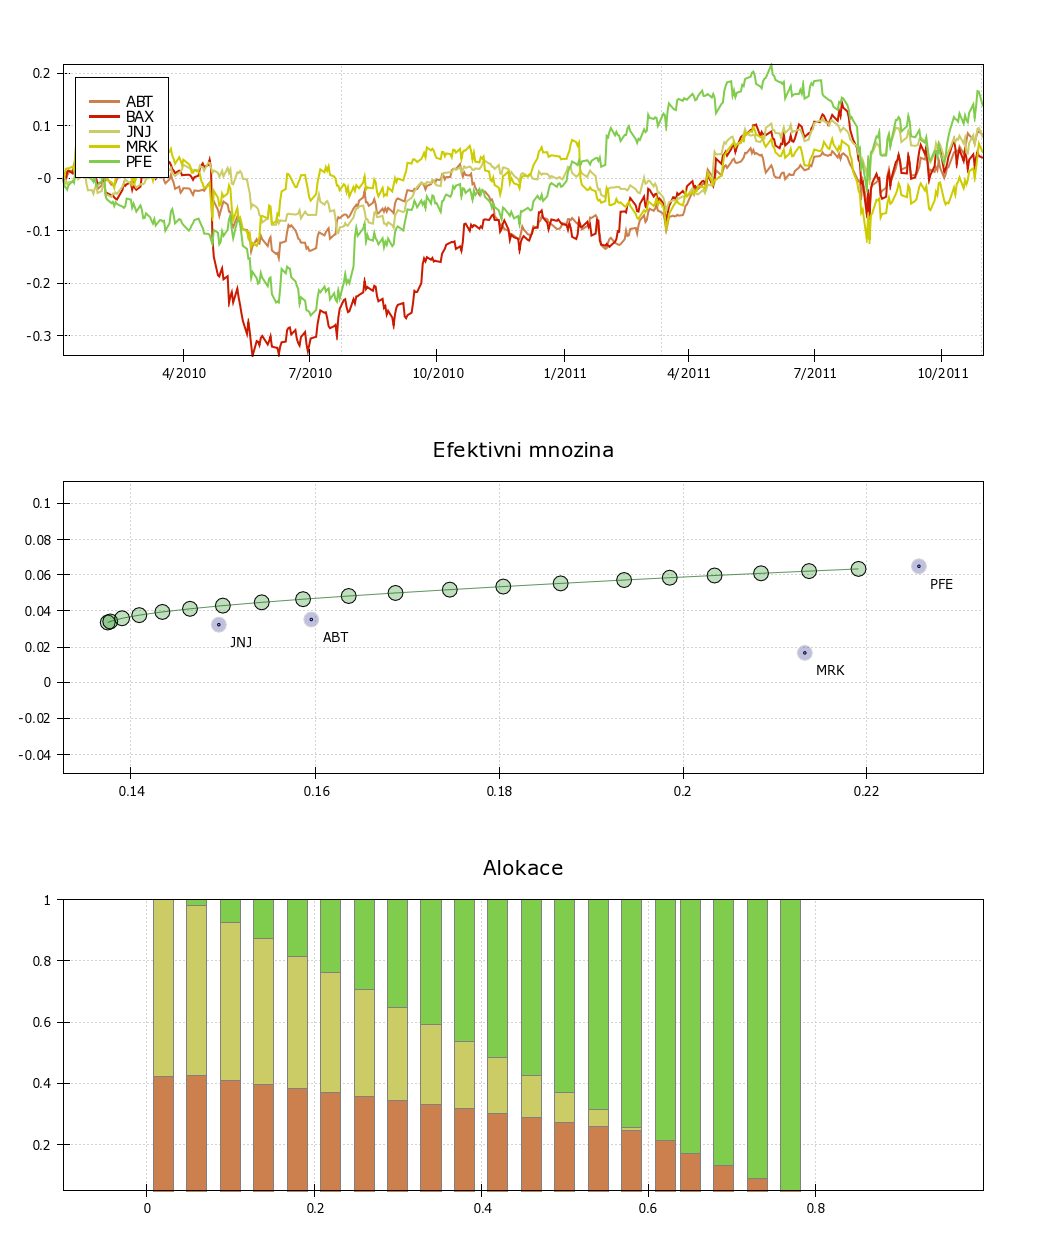
\includegraphics[height=0.9\textheight]{drugs1.png}
\end{frame}

\begin{frame}{Portfolio výrobců farmaceutik}
      \begin{tabular}{|l|l|r|}
        \hline
        Symbol&Název&Alokace\\\hline\hline
        ABT&Abbott Labs &0.424\\\hline
        JNJ&Johnson \& Johnson &0.576\\\hline
      \end{tabular}
      
      Výnos 3.359\%\\
      Volatilita 0.137
\end{frame}

\begin{frame}{Finanční sektor}
      \begin{tabular}{|l|l|r|r|}
        \hline
        Symbol&Název&Volatilita&Roční výnos\\\hline\hline
        AXP&American Express &0.315&17.55\%\\\hline
        BAC&Bank of America Corp. &0.479&-34.62\%\\\hline
        C&Citigroup Inc. &0.445&5.03\%\\\hline
        GS&Goldman Sachs Group &0.331&-19.59\%\\\hline
        JPM&JPMorgan Chase \& Co. &0.343&-5.188\%\\\hline
        MS&Morgan Stanley &0.457&-20.4\%\\\hline
        NDAQ&NASDAQ OMX Group &0.352&16.9\%\\\hline
        NYX&NYSE Euronext &0.398&12.58\%\\\hline
      \end{tabular}
\end{frame}

\begin{frame}{Finanční sektor}
        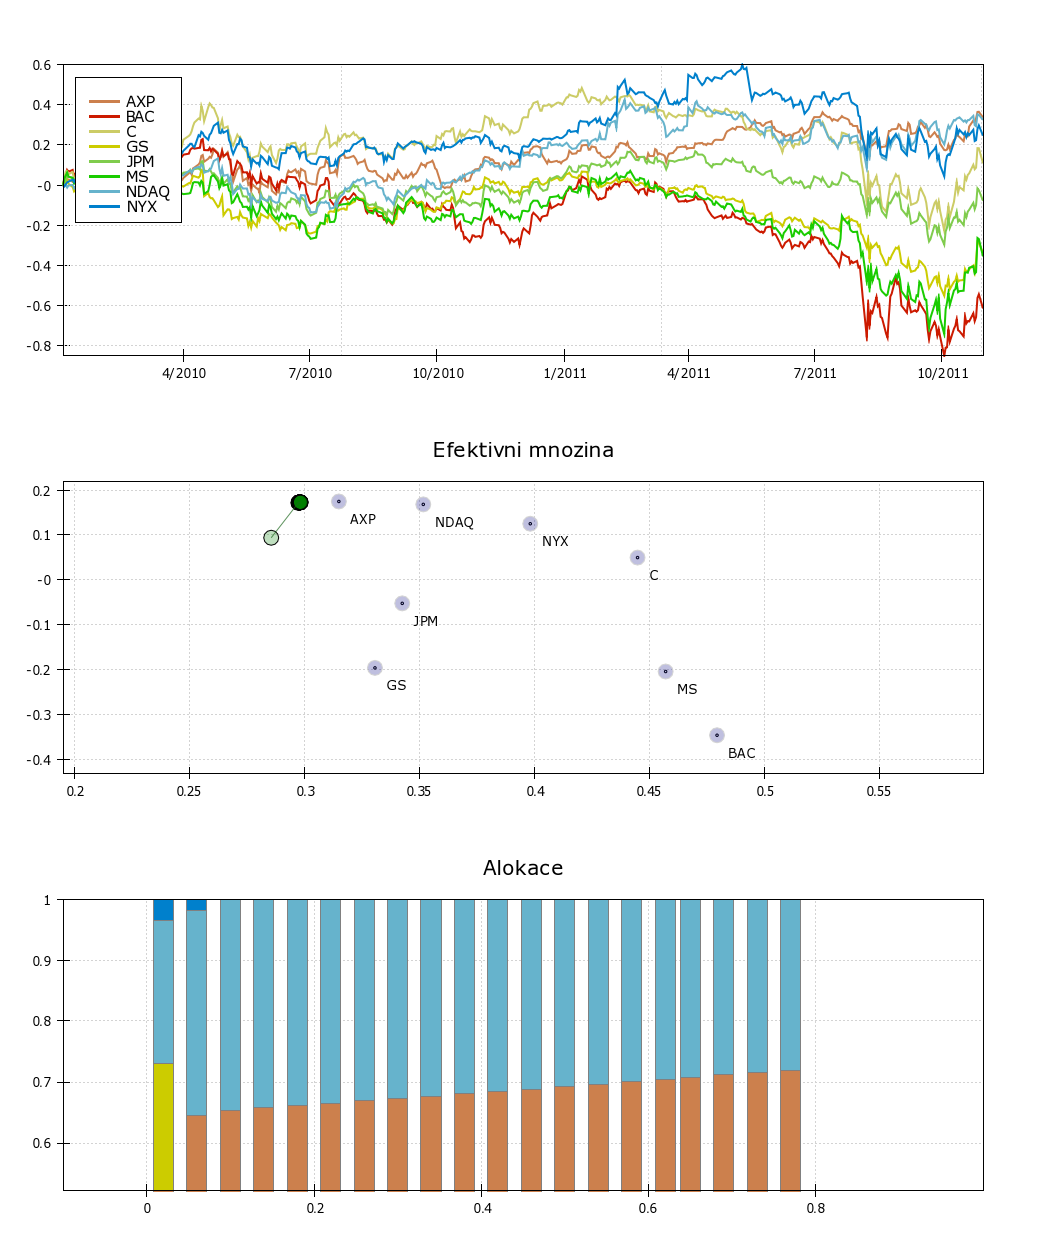
\includegraphics[height=0.9\textheight]{fin1.png}
\end{frame}

\begin{frame}{Finanční sektor}
      \begin{tabular}{|l|l|r|}
        \hline
        Symbol&Název&Alokace\\\hline\hline
        AXP&American Express &0.522\\\hline
        GS&Goldman Sachs Group &0.209\\\hline
        NDAQ&NASDAQ OMX Group &0.235\\\hline
        NYX&NYSE Euronext &0.0341\\\hline
      \end{tabular}
      
      Výnos 9.456\%\\
      Volatilita 0.286
\end{frame}

\begin{frame}{Průmysl}
      \begin{tabular}{|l|l|r|r|}
        \hline
        Symbol&Název&Volatilita&Roční výnos\\\hline\hline
        BA&Boeing Company &0.299&14.5\%\\\hline
        CAT&Caterpillar Inc. &0.34&33.5\%\\\hline
        GE&General Electric &0.286&10.3\%\\\hline
        HON&Honeywell Int'l Inc. &0.29&20.14\%\\\hline
        MMM&3M Company &0.24&1.624\%\\\hline
      \end{tabular}
\end{frame}

\begin{frame}{Průmysl}
        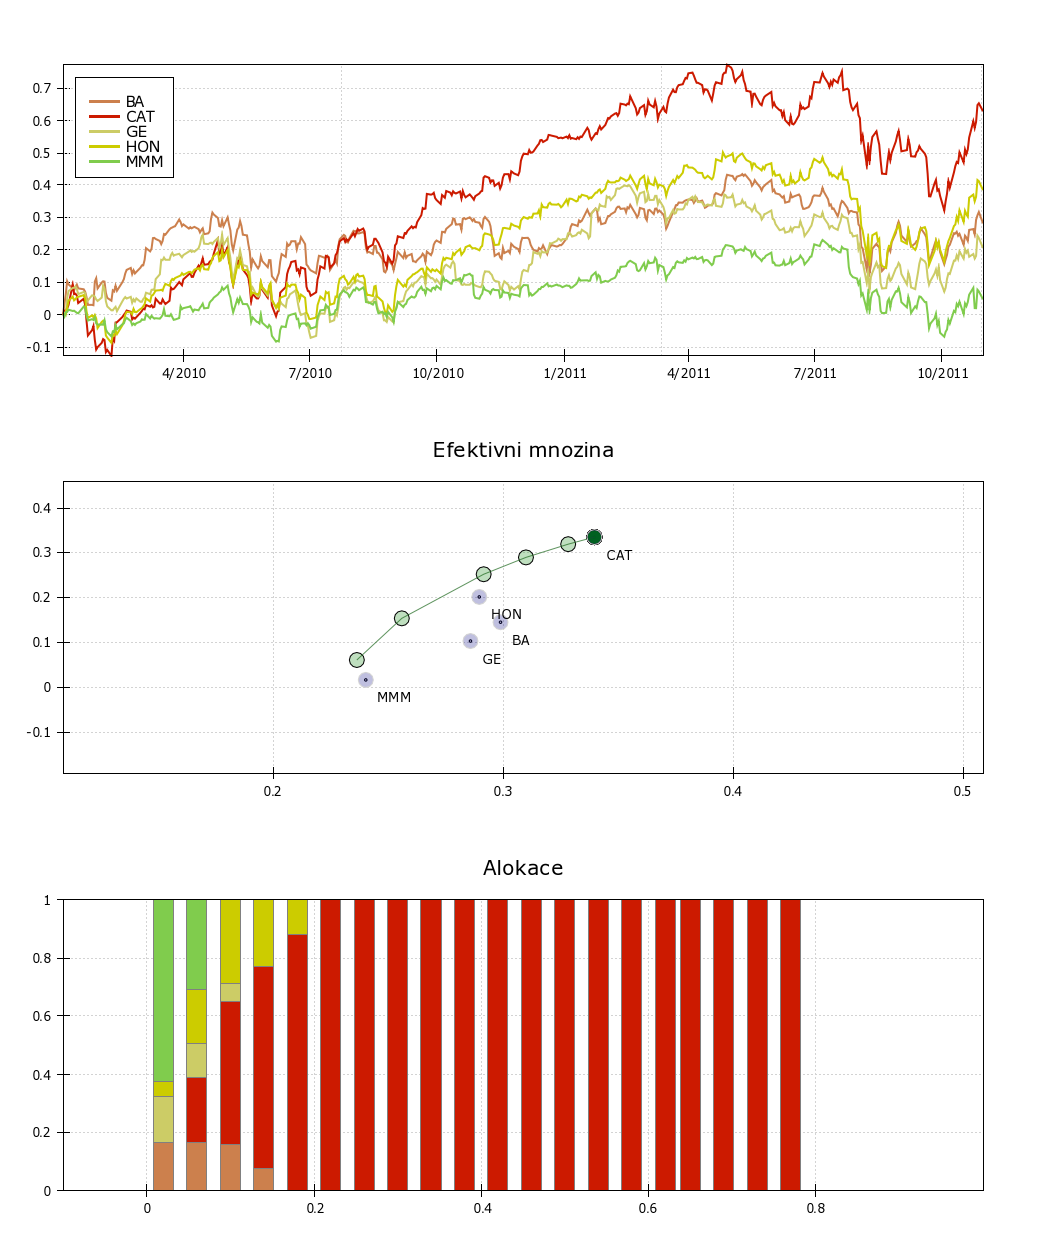
\includegraphics[height=0.9\textheight]{ind1.png}
\end{frame}

\begin{frame}{Průmysl}
      \begin{tabular}{|l|l|r|}
        \hline
        Symbol&Název&Alokace\\\hline\hline
        BA&Boeing Company &0.165\\\hline
        GE&General Electric &0.16\\\hline
        HON&Honeywell Int'l Inc. &0.0501\\\hline
        MMM&3M Company &0.624\\\hline
      \end{tabular}
      
      Výnos 6.073\%\\
      Volatilita 0.236
\end{frame}

\begin{frame}{Nejcennější značky}
10 nejcennějších značek podle Financial Times\cite{ft}\\ 
      \begin{tabular}{|l|l|r|r|}
        \hline
        Symbol&Název&Volatilita&Roční výnos\\\hline\hline
        AAPL&Apple Inc. &0.266&37.57\%\\\hline
        GE&General Electric &0.286&10.3\%\\\hline
        GOOG&Google Inc. &0.291&0.1524\%\\\hline
        IBM&International Bus. Machines &0.198&20.96\%\\\hline
        KO&Coca Cola Co. &0.164&13.13\%\\\hline
        MCD&McDonald's Corp. &0.161&24.78\%\\\hline
        MO&Altria Group Inc. &0.157&24.47\%\\\hline
        MSFT&Microsoft Corp. &0.226&-4.513\%\\\hline
        T&AT\&T Inc. &0.166&8.371\%\\\hline
        VZ&Verizon Communications &0.18&12.74\%\\\hline
      \end{tabular}
\end{frame}

\begin{frame}{Nejcennější značky}
        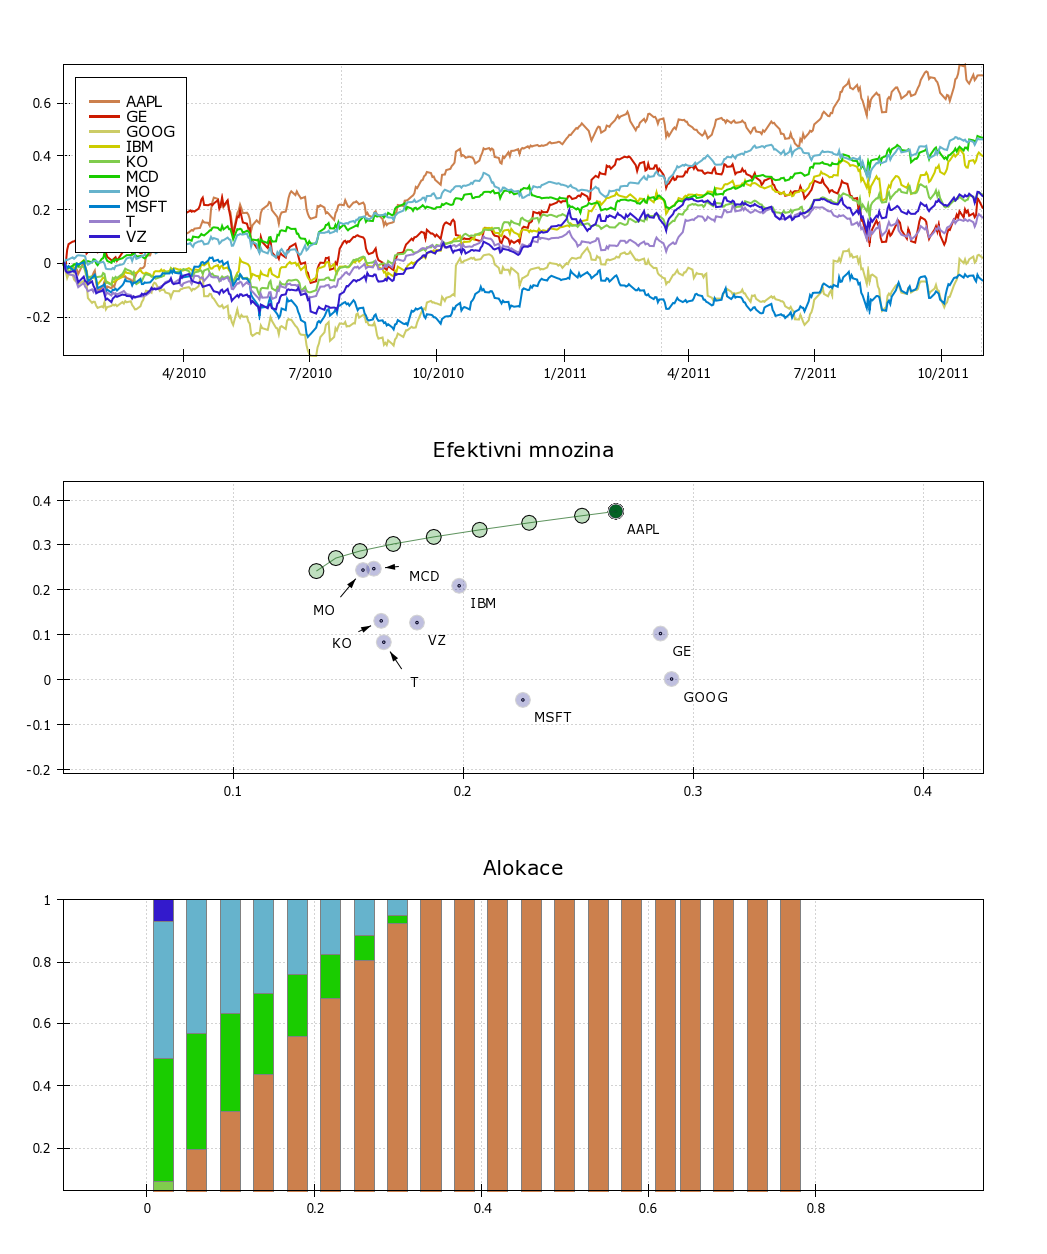
\includegraphics[height=0.9\textheight]{brands1.png}
\end{frame}

\begin{frame}{Nejcennější značky}
      \begin{tabular}{|l|l|r|}
        \hline
        Symbol&Název&Alokace\\\hline\hline
        AAPL&Apple Inc. &0.0617\\\hline
        KO&Coca Cola Co. &0.0311\\\hline
        MCD&McDonald's Corp. &0.394\\\hline
        MO&Altria Group Inc. &0.444\\\hline
        VZ&Verizon Communications &0.0688\\\hline
      \end{tabular}
      
      Výnos 24.24\%\\
      Volatilita 0.136
\end{frame}

\begin{frame}{Deset nejziskovějších titulů}
      \begin{tabular}{|l|l|r|r|}
        \hline
        Symbol&Název&Volatilita&Roční výnos\\\hline\hline
        ACAS&American Capital Strategies Ltd &0.502&72.66\%\\\hline
        AN&AutoNation Inc. &0.352&43.83\%\\\hline
        ANF&Abercrombie \& Fitch Co. &0.457&52.22\%\\\hline
        BIIB&BIOGEN IDEC Inc. &0.303&46.06\%\\\hline
        CMI&Cummins Inc. &0.417&50.12\%\\\hline
        EL&Estee Lauder Cos. &0.317&43.38\%\\\hline
        EP&El Paso Corp. &0.39&55.31\%\\\hline
        FDO&Family Dollar Stores &0.302&46.62\%\\\hline
        LTD&Limited Brands Inc. &0.346&50.85\%\\\hline
        MBI&MBIA Inc. &0.644&60.09\%\\\hline
      \end{tabular}
\end{frame}

\begin{frame}{Deset nejziskovějších titulů}
        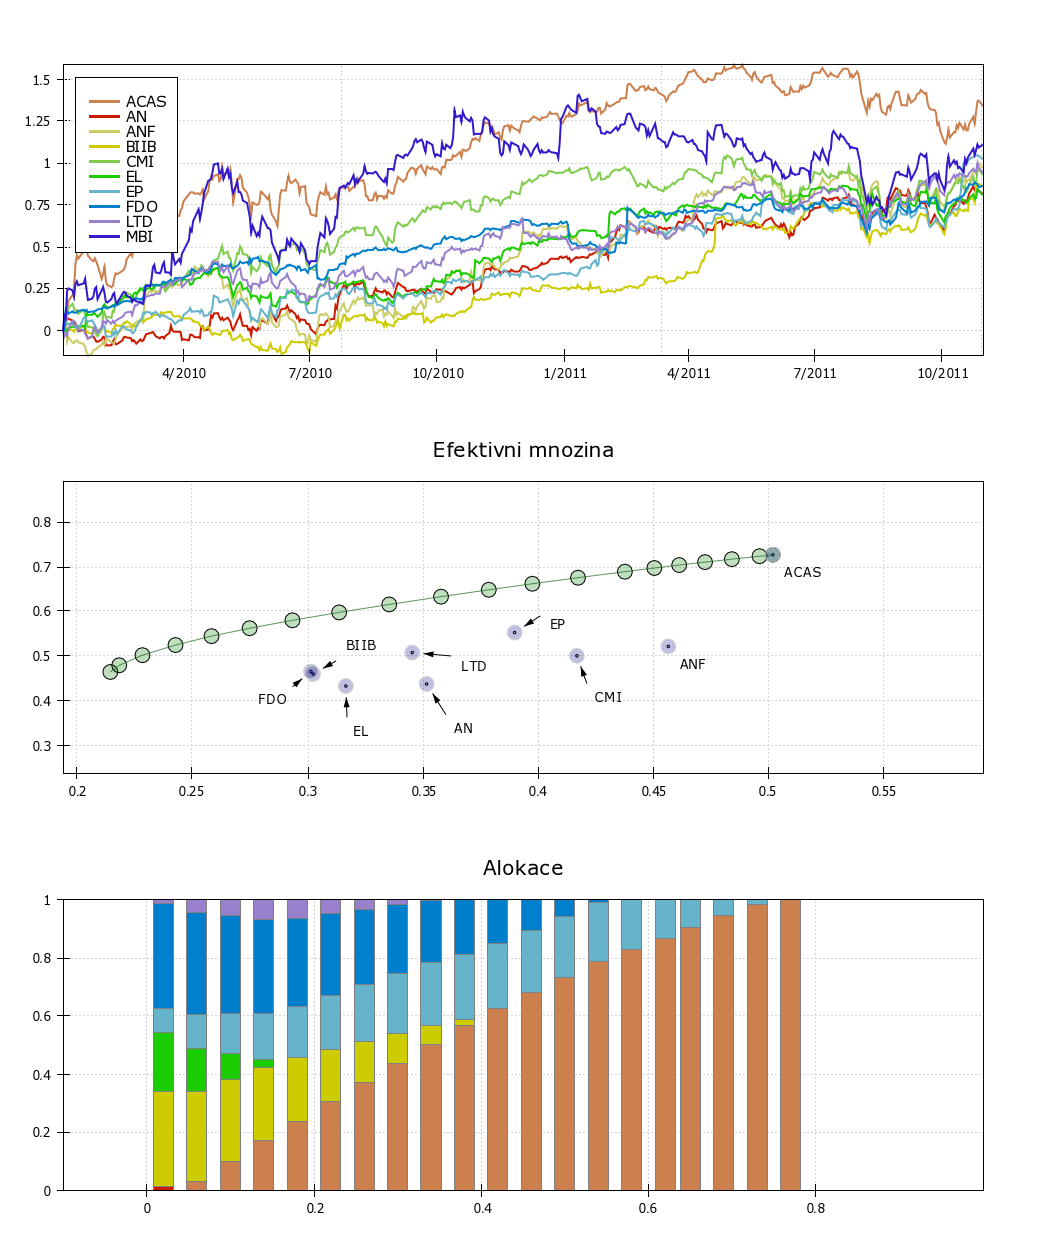
\includegraphics[height=0.9\textheight]{top10.png}
\end{frame}

\begin{frame}{Deset nejziskovějších titulů}
      \begin{tabular}{|l|l|r|}
        \hline
        Symbol&Název&Alokace\\\hline\hline
        AN&AutoNation Inc. &0.0163\\\hline
        BIIB&BIOGEN IDEC Inc. &0.326\\\hline
        EL&Estee Lauder Cos. &0.201\\\hline
        EP&El Paso Corp. &0.0828\\\hline
        FDO&Family Dollar Stores &0.36\\\hline
        LTD&Limited Brands Inc. &0.014\\\hline
      \end{tabular}
      
      Výnos 46.52\%\\
      Volatilita 0.214
\end{frame}

\begin{frame}[shrink=15]{Celý S\&P500} 
      \begin{tabular}{|l|l|r|r|r|}
        \hline
        Symbol&Název&Alokace&Volatilita&Roční výnos\\\hline\hline
        AZO&AutoZone Inc. &0.287&0.177&39.94\%\\\hline
        BIIB&BIOGEN IDEC Inc. &0.0446&0.303&46.06\%\\\hline
        FDO&Family Dollar Stores &0.0744&0.302&46.62\%\\\hline
        HSY&The Hershey Company &0.127&0.198&28.72\%\\\hline
        MCD&McDonald's Corp. &0.0317&0.161&24.78\%\\\hline
        MO&Altria Group Inc. &0.105&0.157&24.47\%\\\hline
        NEM&Newmont Mining Corp. (Hldg. Co.) &0.0161&0.3&22.29\%\\\hline
        SO&Southern Co. &0.315&0.129&19.01\%\\\hline
      \end{tabular}
      
      Výnos 30.32\%\\
      Volatilita 0.119
\end{frame}



  
  \renewcommand{\bibname}{Seznam použité literatury}
  \begin{frame}[shrink=15]
    \frametitle{Seznam použité literatury}
    \begin{thebibliography}{9}
      \addcontentsline{toc}{chapter}{Seznam použité literatury}
      %\thispagestyle{plain}
      \bibitem{camsky}
        ČÁMSKÝ, František. \emph{Teorie portfolia.} 2. přeprac. a rozš. vyd. Brno : Masarykova univerzita, 2007. 115 s. ISBN 9788021042520.
      \bibitem{markowitz}
        MARKOWITZ, Harry. \emph{Portfolio Selection.} The Journal of Finance. Mar., 1952, Vol. 7, No. 1, s. 77-91.
        
      \bibitem{tvaught}
      VAUGHT, Travis. Travis Vaught Blog [online]. 2011-09-01 [cit. 2011-11-26]. Modern Portfolio Theory - A Python Implementation. Dostupné z WWW: \url{http://travisvaught.blogspot.com/2011/09/modern-portfolio-theory-python.html}.

      \bibitem{source}
      VAUGHT, Travis. GitHub [online]. 2009-10-31 [cit. 2011-11-26]. Portfolio metrics. Dostupné z WWW: \url{https://github.com/tvaught/experimental/tree/master/portfolio_metrics}.

      \bibitem{sharpe}
      SHARPE, William F., William F. Shapre personal page [online]. 2008 [cit. 2011-11-26]. The Gradient Method. Dostupné z WWW: \url{http://www.stanford.edu/~wfsharpe/mia/opt/mia_opt1.htm}.

      \bibitem{yahoo}
      Yahoo! Inc. Yahoo! Finance [online]. c2011 [cit. 2011-11-26]. Dostupné z WWW: \url{http://finance.yahoo.com/}.

      \bibitem{ft}
      Finacial Times. Financial Times Special Report [online]. 2011-05-19 [cit. 2011-11-26]. Global Brands. Dostupné z WWW: \url{http://www.millwardbrown.com/Libraries/Optimor_BrandZ_Files/2011_BrandZ_FinancialTimes_SpecialReport.sflb.ashx}.
    \end{thebibliography}
  \end{frame}
\end{document}
